
%(BEGIN_QUESTION)
% Copyright 2008, Tony R. Kuphaldt, released under the Creative Commons Attribution License (v 1.0)
% This means you may do almost anything with this work of mine, so long as you give me proper credit

Calculate the proper $C_v$ value for this valve, given the flow rate and pressures shown for full-open condition.  Assume the process liquid is ethanol (density = 49.3 lb/ft$^{3}$):

$$\includegraphics[width=15.5cm]{i03217x01.eps}$$

Also, calculate the approximate pipe size of control valve necessary to achieve this flow capacity, assuming the use of a double-ported globe valve with a ported plug ($C_d$ = 12.5).

\underbar{file i03217}
%(END_QUESTION)





%(BEGIN_ANSWER)

$C_v$ = 65.6
 
\vskip 10pt

A 2.5 inch control valve should be sufficient.

%(END_ANSWER)





%(BEGIN_NOTES)

$C_d$ = 2.29, rounded up to 2.5 inches nominal.

%INDEX% Final Control Elements, valve: sizing

%(END_NOTES)


